
\section{Metodologia para Reconstrução de Processos}

Uma vez ouvi a seguinte frase dita por Gustavo Caetano\footnote{CEO da SambaTech} que nunca mais saiu de minha mente:
\begin{quote}
    \textbf{SE} você me traz um problema \\
    \textbf{MAS} não me traz a solução \\
    \textbf{ENTÃO} você faz parte do problema
\end{quote}

Depois de refletir por muito tempo, entendi que nem sempre sabemos a solução de todos os problemas assim quando nos deparamos com eles e que  todos devem ser reportados imediatamente para mitigar quaisquer efeitos negativos. Por isso, adaptei essa frase para algo um pouco mais tangível:
\begin{quote}
    \textbf{SE} você me traz um problema \\
    \textbf{ENTÃO} vamos discutir uma solução \\
    \textbf{POIS} juntos trabalhamos melhor
\end{quote}

Baseado nessa frase, gostaria de apresentar uma metodologia ágil que estou desenvolvendo para reconstrução de processos maduros a qual batizei de \textbf{AIOROS}. Por mais caricata ou incomum que pareça, esta metodologia foi baseada na série japonesa de mangá e anime chamada \textbf{Os Cavaleiros do Zodíaco} veiculada no Brasil por volta dos anos 90.

Apesar de possuir diversas sagas, a primeira nos interessa por fazer uma analogia quase perfeita para o contexto que precisamos, onde os cavaleiros de bronze precisam salvar a princesa ferida, correndo contra to tempo, e para isso precisam passar pelas 12 casas do zodíaco enfrentando seus guardiões.

\begin{figure}[H]
    \centering
    
\includegraphics[scale=0.33,keepaspectratio=true]{images/06.png}
    \caption{Saori, reencarnação de Athena, ferida}
\end{figure}

Adaptando essa estória para nossa realidade, imagine que a princesa Saori seja a empresa ou o processo que está em execução de forma legada, ou seja, apenas com seu metabolismo basal não sendo capaz de entregar nada além do que suas funções básicas.

\begin{figure}[H]
    \centering
    
\includegraphics[scale=0.33,keepaspectratio=true]{images/05.jpg}
    \caption{Os Cavaleiros de Bronze}
\end{figure}

Já os cavaleiros de prata são os funcionários que reconhecem essa fraqueza nos processos legados e lutam arduamente em suas casas, enfrentando um guardião por vez.

\begin{figure}[H]
    \centering
    
\includegraphics[scale=0.35,keepaspectratio=true]{images/07.png}
    \caption{Relógio das 12 casas do Zodíaco}
\end{figure}

O Relógio do Zodíaco a agilidade, ou seja, o time não tem muito tempo a perder pois processos e clientes aguardam ansiosamente por melhorias e o time deve trabalhar de forma integrada, coesa, a fim de garantir entregar dentro do prazo.

\begin{figure}[H]
    \centering
    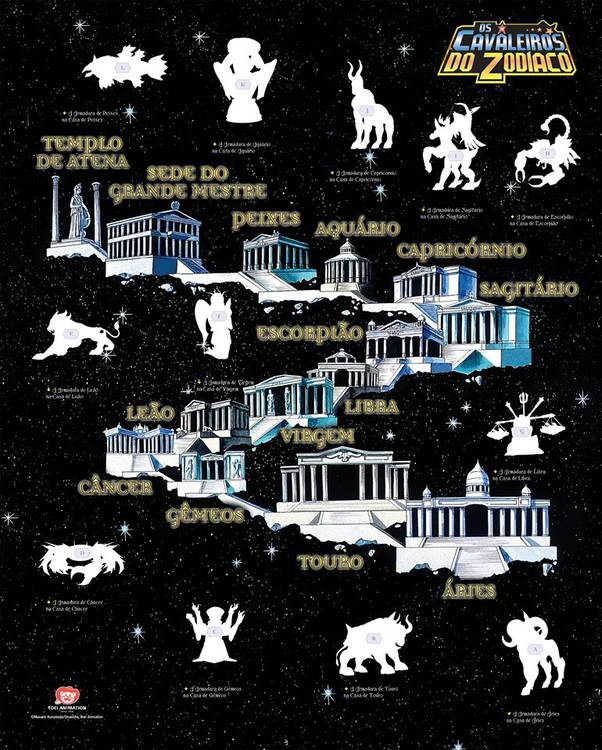
\includegraphics[scale=0.55,keepaspectratio=true]{images/08.jpg}
    \caption{As 12 casas do Zodíaco}
\end{figure}

As 12 Casas do Zodíaco representam em quantas partes o processo como um todo deverá ser quebrado. Deste ponto de vista, faz mais sentido dizer \textbf{As \emph{n} Casas do Zodíaco}. Mas aqui vale uma ressalva: 
\begin{itemize}
    \item Poucas casas deixam o sistema muito coeso, de difícil manutenção e com Cavaleiros de mais para combater
    \item Muitas casas deixar o sistema muito esparso, de difícil manutenção e com Cavaleiros de menos para combater
\end{itemize}

O segredo é ter uma equipe experiente para se definir qual é o número ideal de casas.

Portanto, vamos ver como isso funcionaria na prática
\begin{enumerate}
    \item Em uma reunião inicial a fim de explicar a todos os interessados o que será feito daqui pra frente;
    \item Em uma segunda reunião, de preferência com os membros mais experientes, deve-se de definir quais serão as casas a serem atacadas bem como nomear seus guardiões\footnote{deve-se haver pelo menos 2 guardiões para que haja uma cooperação mútua}
    \item Os guardiões, de posse de suas casas, devem definir os critérios de aceite e as regras de negócio que acharem pertinente à sua casa.
    \item Agora é a vez dos cavaleiros utilizarem do que há de melhor, elevando seus cosmos ao sétimo sentido, propondo soluções engenhosas que capazes de cobrir tudo que foi proposto pelos guardiões daquela casa. 
    \item Neste momento, Product Managers, Designers e Writers atuam ativamente na composição da solução do produto.
    \item Estes passos devem ser repetidos até que todo o projeto tenha finalizado. 
    \item Agora, Product Managers, Designers e Writers devem dar um formato no projeto, adicionando Epic, Estória, Tarefa, Sub-Tarefa para que os times executantes possam indicar o esforço para cada tarefa descrita. 
    \item Writers, não se esqueçam de que faz parte da entrega todas as chaves estarem traduzidas quando o projeto estiver fechado, ou seja, o time de desenvolvimento não poderá iniciar qualquer tarefa desde que essa condição não seja satisfeita. Essa entrega pode ser feita até via arquivo de texto anexado no card do jira, por exemplo.
    \item Voltando a falar sobre mensurar, como já teremos nosso livro de referência, teremos uma grande noção do quanto dura cada atividade, pelo menos uma boa aproximação. Dessa forma, fica bem mais simples e preciso saber quando uma tarefa deverá ser finalizada.
\end{enumerate}
